\documentclass[%
 reprint,
%superscriptaddress,
%groupedaddress,
%unsortedaddress,
%runinaddress,
%frontmatterverbose, 
%preprint,
%showpacs,preprintnumbers,
%nofootinbib,
%nobibnotes,
%bibnotes,
 amsmath,amssymb,
 aps,
%pra,
%prb,
%rmp,
%prstab,
%prstper,
%floatfix,
]{revtex4-1}

\usepackage{graphicx}% Include figure files
\usepackage{dcolumn}% Align table columns on decimal point
\usepackage{bm}% bold math
%\usepackage{hyperref}% add hypertext capabilities
%\usepackage[mathlines]{lineno}% Enable numbering of text and display math
%\linenumbers\relax % Commence numbering lines

%\usepackage[showframe,%Uncomment any one of the following lines to test 
%%scale=0.7, marginratio={1:1, 2:3}, ignoreall,% default settings
%%text={7in,10in},centering,
%%margin=1.5in,
%%total={6.5in,8.75in}, top=1.2in, left=0.9in, includefoot,
%%height=10in,a5paper,hmargin={3cm,0.8in},
%]{geometry}

\usepackage{cmap} % Поиск в PDF
\usepackage[T2A]{fontenc} % Кодировка
\usepackage[utf8]{inputenc} % Кодировка исходного текста
\usepackage[english, russian]{babel} % Локализация и переносы
\frenchspacing % Более тонкая настройка пробелов 
\usepackage{multirow}
\usepackage[warn]{mathtext}
\usepackage{amssymb}
\usepackage{ dsfont }

% Переопределение англоязычного начертания каппа, фи и эпсилон, 
% а также знаков сравнения
\renewcommand{\epsilon}{\ensuremath{\varepsilon}}
\renewcommand{\phi}{\ensuremath{\varphi}} 
\renewcommand{\kappa}{\ensuremath{\varkappa}}
\renewcommand{\le}{\ensuremath{\leslant}}
\renewcommand{\leq}{\ensuremath{\leqslant}}
\renewcommand{\ge}{\ensuremath{\geslant}}
\renewcommand{\geq}{\ensuremath{\geqslant}}
\renewcommand{\emptyset}{\ensuremath{\varnothing}}

\usepackage{textcomp} 
\usepackage{indentfirst} % Красная строка
\usepackage{amsmath} % Текст в формулах
\usepackage{graphicx} % Графика
\DeclareGraphicsExtensions{.pdf,.png,.jpg}
\usepackage{pgfplots}
\pgfplotsset{compat=1.13}

%\usepackage{times}

\begin{document}

\title{Исследование гальванометра}
\thanks{3.2.6}

\author{Иван Едигарьев,}
\affiliation{
 Московский Физико-Технический Институт\\
 Факультет Общей и Прикладной Физики, 526т\\
}
%\date{\today}

\begin{abstract}
Цель работы: изучение работы высокочувствительного зеркального гальванометра магнитоэлектрической системы в режимах измерения постоянного тока и электрического заряда.

В работе используются: зеркальный гальванометр с осветителем и шкалой, источник постоянного напряжения, делитель напряжения, магазин сопротивлений, эталонный конденсатор, вольтметр, переключатель, ключи, линейка.\\

\end{abstract}

\pacs{Valid PACS appear here}% PACS, the Physics and Astronomy
                             % Classification Scheme.
%\keywords{Suggested keywords}%Use showkeys class option if keyword
                              %display desired
\maketitle

%\tableofcontent

\section{\label{sec:level1}Определение динамической постоянной}

\begin{figure}[h]
\center{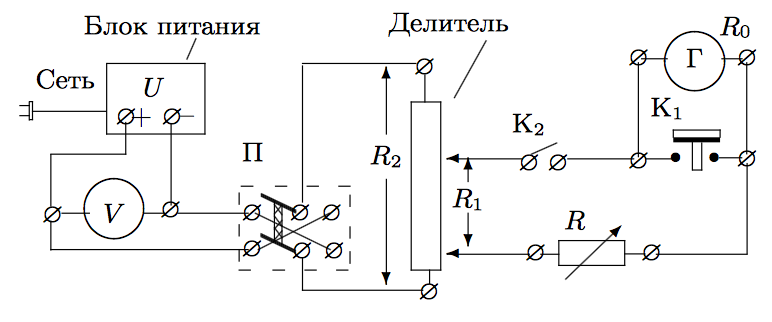
\includegraphics[scale=0.27]{pic1.png}}
\caption{Схема установки для работы гальванометра в стационарном режиме}
\end{figure}

\textbf{Экспериментальная установка.} Схема для исследования гальванометра в стационарном (или динамическом) режиме представлена на рис.1. Постоянное напряжение $U \simeq 1,5$ В снимается с блока питания и измеряется вольтметром $V$. Ключ П позволяет менять направление тока через гальванометр Г, делитель напряжения — менять величину тока в широких пределах. Ключ П служит для включения гальванометра, кнопка $\text{K}_1$ — для его успокоения. Магазин сопротивлений $R$ позволяет менять режим работы гальванометра от колебательного до апериодического.

При малых $R_1$ сила тока, протекающего через гальванометр может быть вычислена по очевидной формуле:
\begin{equation}
    I = U_0 \frac{R_1}{R_2}\frac{1}{R+R_0},
\end{equation}
где $U_0$ — показания вольтметра, $R_1 / R_2$ — положение делителя, $R$ — сопротивление магазина, $R_0$ — внутреннее сопротивление гальванометра.

Угол отклонения рамки от положения равновесия измеряется с помощью осветителя, зеркальца, укреплённого на рамке, и шкалы, на которую отбрасывается луч света от зеркальца. Координата $x$ светового пятна на шкале связана с углом отклонения рамки формулой
$$ x = a \tg(2 \phi),$$
где $a$ — расстояние от шкалы до зеркальца. При малых углах можно считать, что $\phi = x/2a$. Динамическую постоянную
\begin{equation}
    C_I = \frac{I}{x / 2a},
\end{equation}
как правило, выражают в единицах $\left[\frac{\text{A}}{\text{мм/м}}\right]$ (ток $I$ измеряется в амперах, $x$ — в мм, $a$ — в метрах). Расстояние $a$ обычно около метра, поэтому величина $C_I$ определяет ток, при котором зайчик отклоняется на одно деление (1 мм).

\section{\label{sec:level1}Определение критического сопротивления гальванометра, работающего в динамическом режиме}

Измерение критического сопротивления гальванометра можно выполнить с помощью той же цепи (рис.1).

При больших $R$ свободное движение рамки имеет колебательный характер. С уменьшением $R$ затухание увеличивается, и колебательный режим переходит в апериодический.

Скорость затухания колебаний принято характеризовать декрементом затухания $\Delta$, равным отношению углов двух последовательных отклонений в одну сторону. Легко показать, что:
$$ \Delta = \frac{\phi_n}{\phi_{n+1}} = \frac{x_n}{x_{n+1}} = e^{\gamma T},$$
где $T$ - период колебаний:
\begin{equation}
    T = \frac{2 \pi}{\omega}.
\end{equation}

Вместо декремента затухания $\Delta$ можно рассматривать логарифмический декремент затухания $\Theta$:
\begin{equation}
    \Theta = \ln \Delta = \gamma T = \ln \frac{x_n}{x_{n+1}}.
\end{equation}

Измеряя зависимость логарифмического декремента затухания от сопротивления внешней цепи, можно найти $R_{\text{кр}}$, т. е. значение $R$, при котором 
$\Theta \rightarrow \infty$. Измерения логарифмического декремента при сильном затухании затруднены, поэтому исследуем зависимость $\Theta$ от $R$. Подставляя в (4) значения $T$ из (3), $\omega$, $\gamma$ и $\omega_0$, получим
\begin{equation}
    \Theta = \gamma T = 2 \pi \frac{\gamma}{\omega} = \frac{2 \pi \gamma}{\sqrt{{\omega_0}^2 - \gamma^2}} = \frac{2 \pi R_3}{\sqrt{(R_0 + R)^2 - {R_3}^2}},
\end{equation}
где введено обозначение
\begin{equation}
    R_3 = \frac{(BSN)^2}{2\sqrt{JD}} = R_0 + R_{\text{кр}}.
\end{equation}
После простого преобразования равенства (5) получим
\begin{equation}
    \frac{1}{\Theta^2} = \frac{(R_0 + R)^2}{4 \pi^2 {R_3}^2} - \frac{1}{4 \pi^2}.
\end{equation}
Последнее уравнение, представленное на графике в координатах $X = (R_0 + R)^2,~Y = 1/{\Theta^2}$ имеет вид прямой, угол наклона которой позволяет рассчитать критическое сопротивление:
\begin{equation}
    R_{\text{кр}} = \frac{1}{2 \pi}\sqrt{\frac{\Delta X}{\Delta Y}} - R_0
\end{equation}

\section{\label{sec:level1}Определение баллистической постоянной
и критического сопротивления гальванометра, работающего в баллистическом режиме}

\begin{figure}[h]
\center{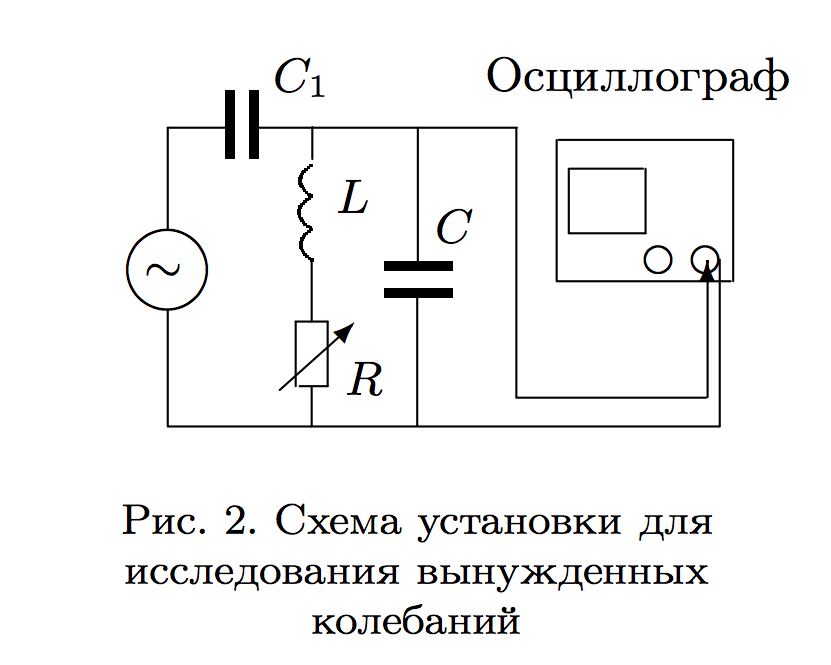
\includegraphics[scale=0.27]{pic2.png}}
\caption{Схема установки для определения баллистической постоянной}
\end{figure}

\textbf{Экспериментальная установка.} Для изучения работы гальванометра в режиме измерения заряда используется схема, представленная на рис. 2. Система ключей устроена так, что нормально ключ $\text{K}_2$ замкнут, а ключи $\text{K}_3$ и $\text{K}_4$ разомкнуты. При нажатии на кнопку $\text{K}_0$ сначала размыкается ключ $\text{K}_2$, затем замыкается $\text{K}_3$ и через некоторое время — $\text{K}_4$.

При нормальном положении кнопки $\text{K}_0$ конденсатор $C$ заряжается до напряжения
$$ U_{\text{C}} = \frac{R_1}{R_2} U_0.$$
Заряд конденсатора равен
\begin{equation}
    q = CU_{\text{C}} = \frac{R_1}{R_2} U_0 C.
\end{equation}

При нажатии на ключ $\text{K}_0$ конденсатор отключается от источника постоянного напряжения (размыкается ключ $\text{K}_2$) и подключается к гальванометру (замыкается ключ $\text{K}_3$).

Ёмкость конденсатора выбрана так, что к моменту замыкания ключа $\text{K}_4$ весь заряд успевает пройти через гальванометр, и рамка получает начальную скорость $\dot{\phi}(\tau)$. При этом можно считать, что отклонение рамки, происходящее за время, протекающее между замыканием ключей $\text{K}_3$ и $\text{K}_4$, равно нулю.

При замыкании ключа $\text{K}_4$ гальванометр шунтируется внешним сопротивлением $R$, и в зависимости от величины этого сопротивления движение рамки описывается одним из уравнений.

Первый отброс зайчика $l_{\text{max}}$ после нажатия на кнопку $\text{K}_0$ зависит от сопротивления внешней цепи, подключённой к гальванометру. Для определения $R_{\text{кр}}$ используется то обстоятельство, что в критическом режиме максимальное отклонение зайчика в $e$ раз меньше, чем у гальванометра без затухания.

Следует помнить, что наблюдать колебания рамки при полном отсутствии затухания, конечно, невозможно, т. к. даже при разомкнутой внешней цепи $(R = \infty)$ остаётся трение в подвеске и трение рамки о воздух. Величину максимального отклонения гальванометра без затухания $\phi_0$ можно, однако, рассчитать, если при разомкнутой цепи измерены максимальное отклонение рамки $\phi_1$ и логарифмический декремент затухания $\Theta_0$.

Легко показать, что
\begin{equation}
    \phi_0 = \phi_1 e^{{\Theta_0}/4}~\text{или}~l_0 = l_1 e^{{\Theta_0}/4}.
\end{equation}

Баллистическая постоянная гальванометра $C_{Q_{\text{кр}}}$ $\left[\frac{\text{Кл}}{\text{мм/м}}\right]$ определяется при критическом сопротивлении ($R = R_{\text{кр}})$:
\begin{equation}
    C_{Q_{\text{кр}}} = \frac{q}{\phi_{\text{max~кр}}} = 2a\frac{R_1}{R_2}\frac{U_0 C}{l_{\text{max~кр}}},
\end{equation}
где $l_{\text{max~кр}}$ — величина первого отброса в критическом режиме, выраженная в делениях шкалы (мм), $a$ — расстояние от зеркальца до шкалы, выраженное в метрах, произведение $U_0 C$ — заряд, выраженный в кулонах. 

\section{\label{sec:level1}Задание}

В работе предлагается определить динамическую постоянную, критическое сопротивление и оценить линейность шкалы гальванометра, работающего в стационарном (токовом) режиме; определить критическое сопротивление и баллистическую постоянную гальванометра, работающего в баллистическом режиме (режиме измерения заряда).

1. Соберите электрическую цепь по рис.1 и подготовьте приборы к работе. 

2. Для определения динамической постоянной снимите зависимость отклонения зайчика $x$ от сопротивления магазина $R$, увеличивая сопротивление магазина, но не меняя делителя (8–10 значений).

3. Запишите показания вольтметра $U_0$, положение делителя $R_1/R_2$, величину $R_2$ и внутреннее сопротивление гальванометра $R_0$, указанное на установке.

4. Проведите измерение логарифмического декремента затухания $\Theta_0$ в режиме свободных колебаний.

5. Измерьте период $T_0$ свободных колебаний рамки (приближённо).

6. Определите критическое сопротивление. Для этого подберите \textbf{наибольшее} сопротивление магазина, при котором при размыкании ключа П зайчик не переходит за нулевое значение. Это сопротивление близко к критическому сопротивлению цепи $R_{\text{кр}}$.

7. Для расчёта $\Theta$ проведите измерение отклонений зайчика после размыкания ключа П, увеличивая $R$ от $\simeq~3R_{\text{кр}}$ (близкое целое) до $10 R_{\text{кр}}$.

8. Для исследования работы гальванометра в баллистическом режиме соберите схему по рис.2.

В режиме свободных колебаний (при разомкнутой цепи $R$) определите первый отброс зайчика после замыкания ключа $\text{K}_0$. Подберите делитель так, чтобы при замыкании ключа $\text{K}_0$ первый отброс $l_{\text{max}}$ соответствовал отклонению зайчика почти на всю шкалу.

Вновь подключите магазин $R$. Не меняя положения делителя, снимите зависимость первого отброса от величины $R$ (8–10 значений).

9. Запишите положение делителя $R_1 / R_2$ и значение ёмкости $C$. Измерьте расстояние $a$ от шкалы до зеркальца гальванометра.

\begin{center}
  Обработка результатов
\end{center}

1. Рассчитайте токи $I$ по формуле (1) и постройте график $I = f(x)$. Оцените линейность шкалы гальванометра. По наклону прямой рассчитайте динамическую постоянную $C_I$ [A/(мм/м)] по формуле (2).

2. Рассчитайте логарифмический декремент затухания $\Theta_0$ разомкнутого гальванометра по формуле (4).

3. Постройте график $1/{\Theta^2} = f[(R + R_0)^2]$ и по наклону прямой (в области малых $R$) рассчитайте критическое сопротивление по формуле (8).

4. Постройте график $l_{\text{max}} = f[(R_0 + R)^{-1}]$. Определите по графику критическое сопротивление гальванометра [с учётом (10)].

5. Рассчитайте баллистическую постоянную в критическом режиме $C_{Q_{\text{кр}}}$ [Кл/(мм/м)] по формуле (11).

6. Сравните время релаксации $t = R_0 C$ и период свободных колебаний гальванометра $T_0$.

7. Сведите результаты эксперимента в таблицу.

8. Оцените погрешности и сравните полученные значения $R_{\text{кр}}$.

\section{\label{sec:level1}Данные}

Рассчитаем токи $I$ по формуле (1) и построим график зависимости $I = f(x)$:\\
\\
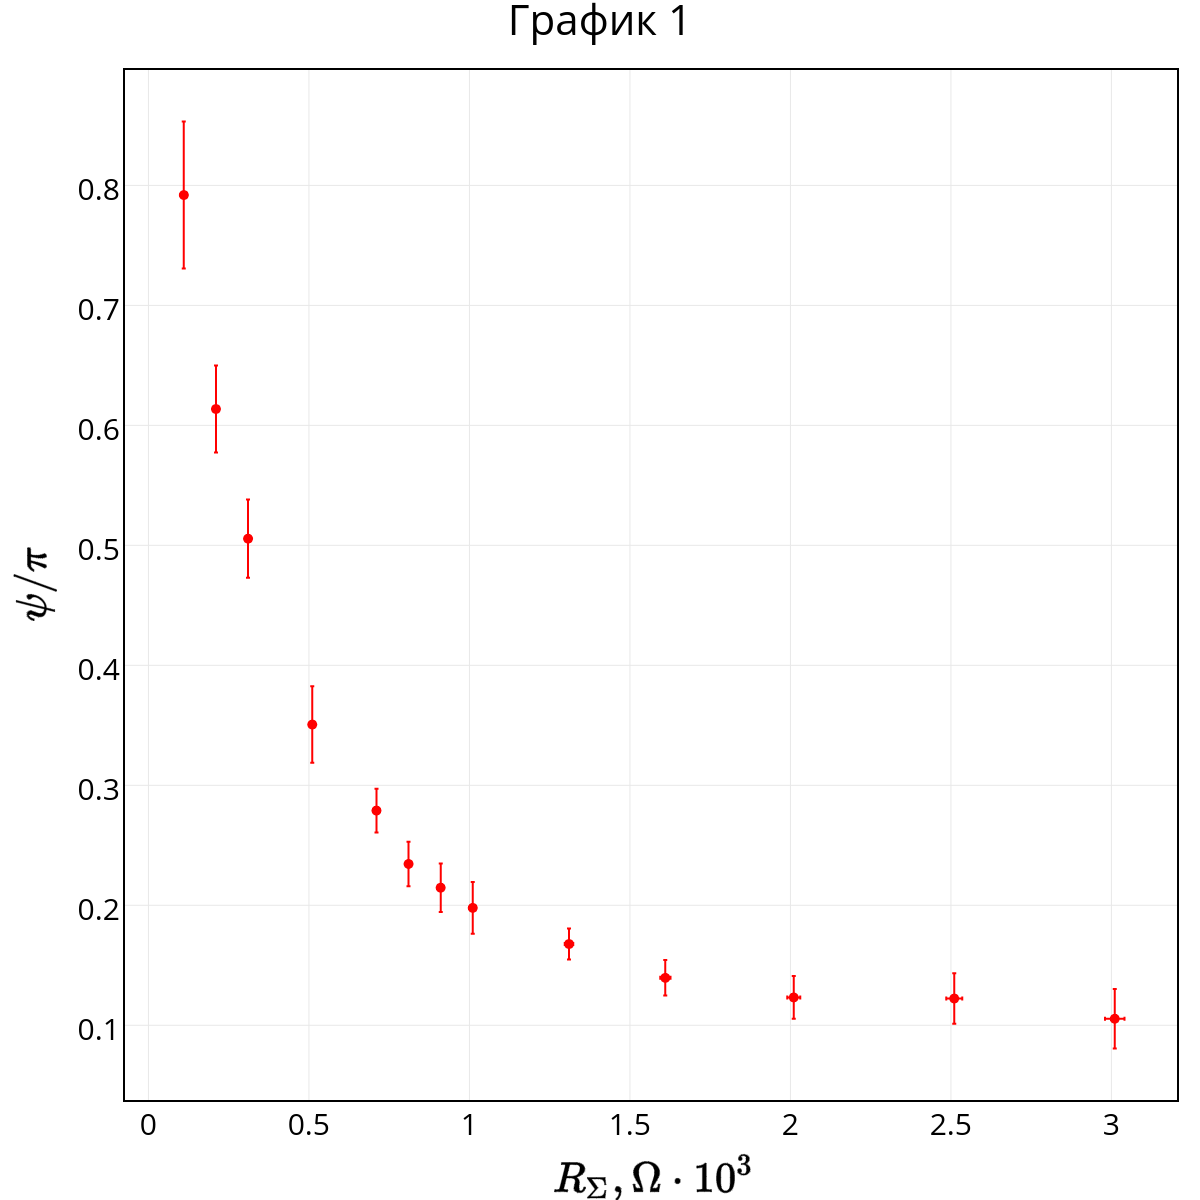
\includegraphics[scale=0.19]{my_plot1.png}\\

Построим линейную регрессию вида $f(x) = \alpha + \beta x$ с квадратичной функцией потерь. По наклону регрессионной прямой рассчитаем динамическую постоянную гальванометра $C_I$ [A/(мм/м)] по формуле (2).
$$ \alpha = (6.0 \pm 0.1^{\text{stat}}),~A \cdot 10^{-9},~~\beta = (3.09 \pm 0.02^{\text{stat}}),~A \cdot 10^{-9} \cdot cm^{-1}$$
$$ C_{I} = 2ka = (77 \pm 2^{\text{syst}}) \cdot 10^{-11}, \frac{A \cdot 10^{-9}~\text{m}}{\text{mm}} $$

По Графику 1 легко видеть, что линейность шкалы гальванометра подтверждается.

Рассчитаем логарифмический декремент затухания $\Theta_0$ разомкнутого гальванометра по формуле (4) и оценим ошибку. Получим:
$$\Theta_0^{12} = 0.30 \pm 0.02^{\text{syst}},~~\Theta_0^{23} = 0.31 \pm 0.03^{\text{syst}},~~\Theta_0 = 0.30 \pm 0.3^{\text{syst}}$$

Измерим период $T_0$ свободных колебаний рамки:
$$ 3T_0 = (18 \pm 1^{\text{syst}})~s,~~T_0 = (6 \pm 0.3^{\text{syst}})~s$$

Подберём наибольшее сопротивление $R$ магазина, при котором зайчик не проходит через нулевое положение. Это сопротивление близко к критическому $R_{\text{кр}}$:
$$ R_{\text{кр}} = (9.4 \pm 0.1^{\text{syst}}),~\Omega \cdot 10^{3}$$

Следующим этапом вычислим значения логарифмического декремента затухания $\Theta$ для соответствующих значений $R$. Построим график $1/{\Theta^2} = f[(R + R_0)^2]$:\\
\\
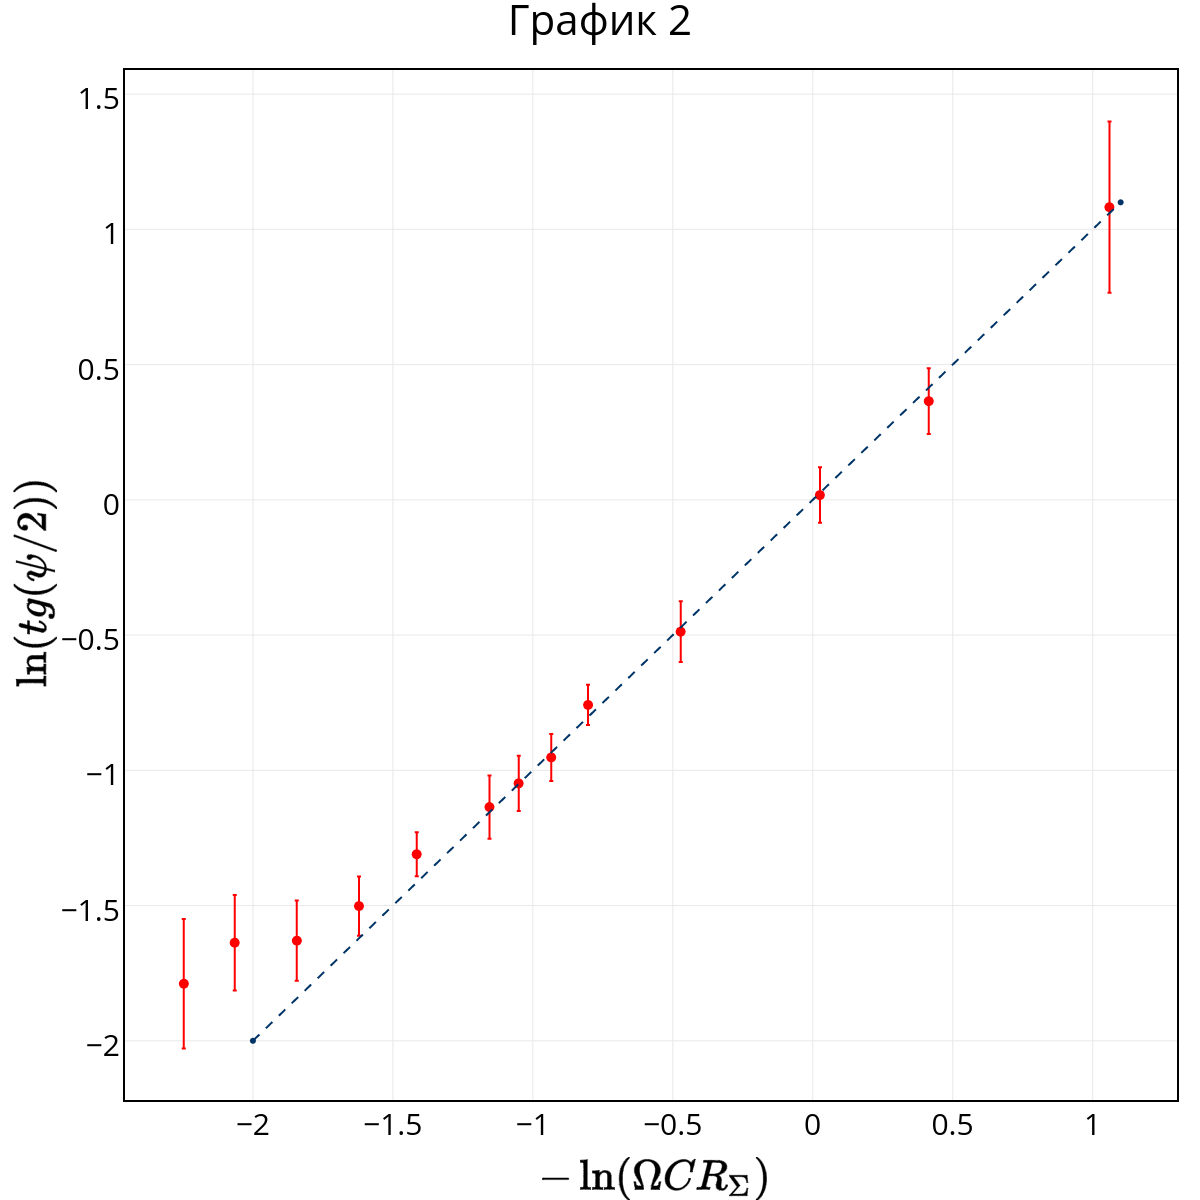
\includegraphics[scale=0.19]{my_plot2.png}\\

Мы предполагаем некоторую линейную зависимость $1/{\Theta^2} = f[(R + R_0)^2]$ (7) в области малых $R$. Построим вариационный ряд измерений по $R$, выберем первые семь точек, и построим по ним линейную регрессию вида $f(x) = \alpha + \beta x$ с квадратичной функцией потерь. Получим:
$$ \alpha = (7 \pm 2^{\text{stat}})~\cdot 10^{-2} ,~~\beta = (26 \pm 1^{\text{stat}}),~\Omega^2 \cdot 10^{-11}$$

Легко видеть, что параметр модели $\alpha$ с точностью до двух значений статистической ошибки согласуется с теоретически предсказанным.

С помощью параметра $\beta$ рассчитаем и оценим ошибку критического сопротивления гальванометра по формуле (8):
$$ R_{\text{кр}} = (9.8 \pm 0.4^{\text{stat}})~\Omega \cdot 10^{3}$$

Теперь проанализируем данные в баллистическом режиме работы гальванометра. Измерим первый отброс зайчика в режиме свободных колебаний:
$$l_{\textbf{max,~св}} = (24.0 \pm 0.1^{\text{syst}})~cm$$

Построим график зависимости $l_{\text{max}} = f[(R_0 + R)^{-1}]$:\\
\\
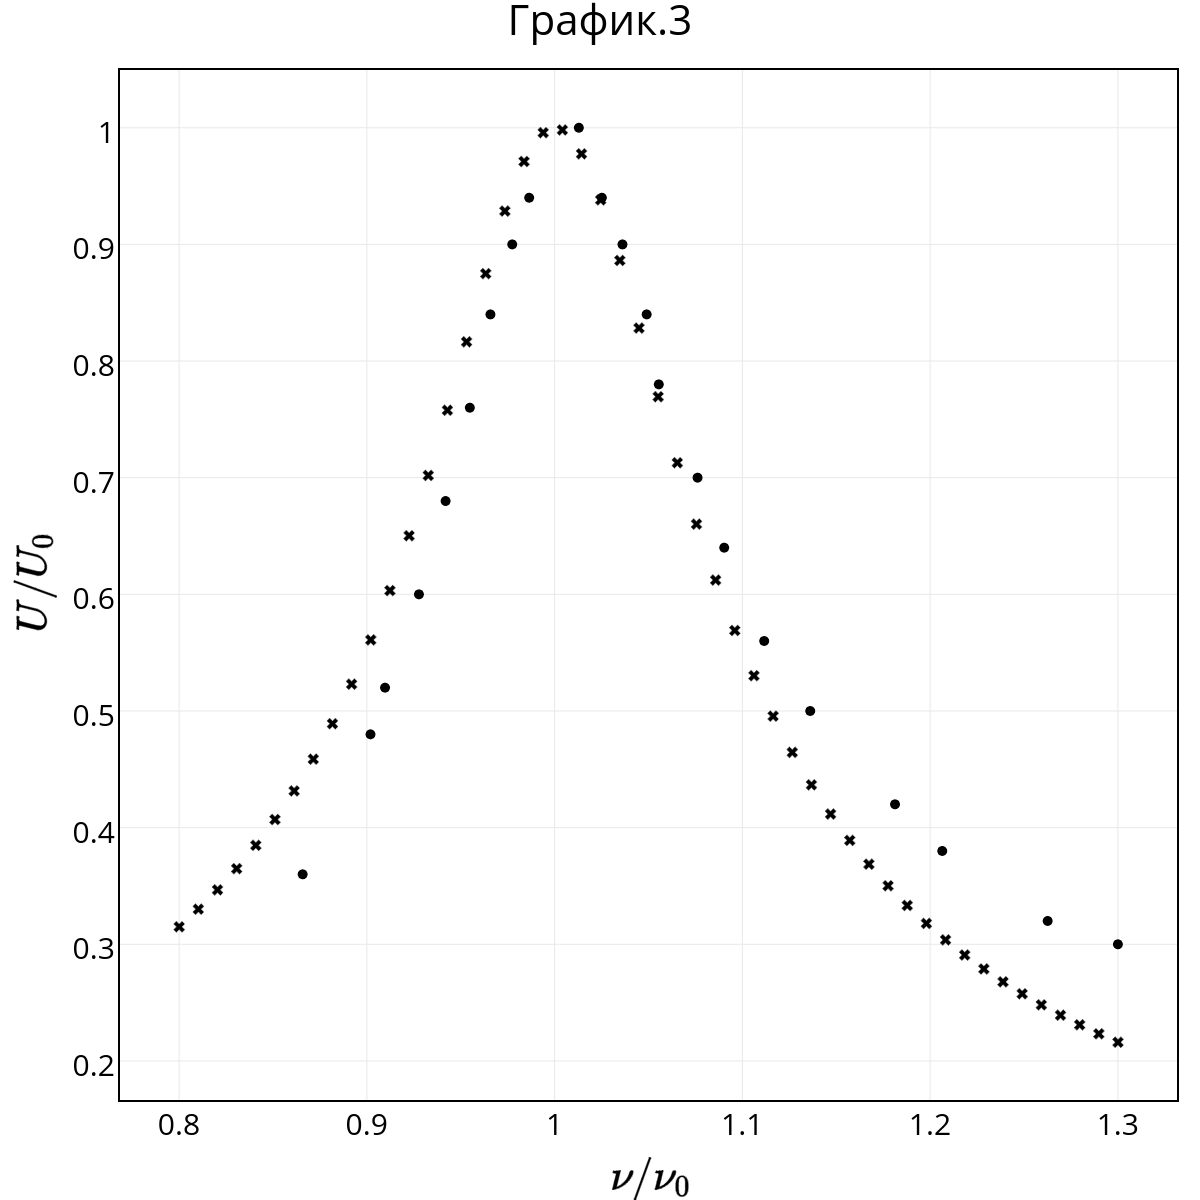
\includegraphics[scale=0.19]{my_plot3.png}\\

Построим трёхпараметрический фит, под зависимость:
$$ f(x) = \alpha + \text{exp}\left[ \beta + \gamma x \right]$$

Получим:
$$\alpha = (4.2\pm 0.2^{\text{stat}})~cm,~~\beta = 2.8 \pm 0.1^{\text{stat}},$$
$$\gamma = (-10.5\pm 0.1^{\text{stat}})~\Omega \cdot 10^{3}$$

Вычислим приблизительное значение $R_{\text{кр}}$ из нашей модели, которое будет соответствовать точке на графике с $l_{\text{max}} = 7.4~cm$:
$$R_{\text{кр}} = (6 \pm 1)~\Omega \cdot 10^{3}$$

Рассчитаем по формуле (11) баллистическую постоянную в критическом режиме $C_{Q_{\text{кр}}}$ [Кл/(мм/м)]:
$$C_{Q_{\text{кр}}} = 2a\frac{R_1}{R_2}\frac{U_0 C}{l_{\text{max~кр}}} = (34.4 \pm 0.2^{\text{syst}})~10^{-10} \frac{C}{mm/m}$$

Оценим время релаксации системы $t$, и сравним это значение с периодом свободных колебаний гальванометра $T_0$:
$$ t \approx R_0 C = 10^{-4}~s~\ll~T_0$$

Как можно видеть, наше рассуждение о том, что в баллистическом режиме можно пренебречь начальным углом и начальной угловой скоростью было верным.

Сведём результаты в итоговую таблицу:\\

\end{document}

